%%%%%%%%%%%%% ptdr definitions %%%%%%%%%%%%%%%%%%%%%
\input{ptdr-definitions}

\newcommand{\pp}{\ensuremath{\mathrm{pp}}}%
\newcommand{\Wo}{\ensuremath{\mathrm{W}}}%
\newcommand{\Zo}{\ensuremath{\mathrm{Z}}}%
\newcommand{\rts}{\ensuremath{\sqrt{s}}}%
\newcommand{\ra}{\ensuremath{\rightarrow}}%
\newcommand{\MN}{\ensuremath{\mu\nu}}%
\newcommand{\MW}{\ensuremath{\mathrm{m}_\Wo}}%
\newcommand{\MZ}{\ensuremath{\mathrm{m}_\Zo}}%
\newcommand{\MT}{\ensuremath{\mathrm{M}_T}}%

\newcommand{\Wmn}{\ensuremath{\Wo \ra \MN}}%
\newcommand{\Zmm}{\ensuremath{\Zo \ra \MM}}%
\newcommand{\Wtn}{\ensuremath{\Wo \ra \tau\nu}}%
\newcommand{\Ztt}{\ensuremath{\Zo \ra \tau\tau}}%
\newcommand{\ppZmm}{\pp \ra \Zo + X \ra \MM + X}%
\newcommand{\ppWmn}{\pp \ra \Wo + X \ra \MN + X}%



%%%%%%%%%%%%%%%  Title page %%%%%%%%%%%%%%%%%%%%%%%%


\cmsNoteHeader{XXX/YYY}


\title{Study of the Barrel RPC L1 Trigger efficiency \\
with a muon sample triggered by the DT system}
% Force line breaks with \\

%Author is always "The CMS Collaboration" for PAS, so author, etc will be ignored
\address[nap]{INFN and Universit{a'} di Napoli}
\address[bari]{INFN and Universita' di Bari}
\author[nap]{F.~Fabozzi}
\author[nap]{A.O.M.~Iorio}
\author[bari]{R.~Trendadue}

% please supply the date in yyyy/mm/dd format. Today has been
% redefined to do so, but it should be fixed as of the final release date.
%\date{\today}

% note that you cannot use \verb in the abstract text
\abstract{
    We present a study of the L1 trigger efficiency for RPCs in the
    Barrel of the CMS Muon System. The method exploits the independency of the
    DT and RPC trigger systems. Muon tracks in the event are 
    triggered and reconstructed using the DT system only, and for each of
    them we search for a compatible RPC L1 trigger object. 
    We discuss in detail the results obtained on a few good 
    runs taken from CRAFT08 and CRAFT09 datasets. The algorithm has been 
    released in the Prompt Analysis Framework of the RPC system for a fast
    off-line monitoring of the trigger performances.
}

% these need to be filled in by hand and should (MUST) match the info
% in the TeX equivalents less the TeX markup
%\hypersetup{%
%pdfauthor={Francesco Fabozzi},%
%pdftitle={Towards a measurement of W and Z cross sections into muons in pp collisions at rts=10 TeV},%
%pdfsubject={CMS},%
%pdfkeywords={CMS, physics, software, computing}}

\maketitle %maketitle comes after all the front information has been supplied

%%%%%%%%%%%%%%%%%%%%%%%%%%%%%%%%  Begin text %%%%%%%%%%%%%%%%%%%%%%%%%%%%%
\section{Introduction}
The CMS Muon System~\cite{ref:mutdr}\cite{ref:jinst} has 
been designed to provide excellent muon
identification, triggering and precise momentum reconstruction 
over the entire kinematic range foreseen at LHC. A crucial
feature of the system is the redundancy provided by the DT/RPC 
(CSC/RPC) independent sub-systems in the Barrel (Endcap) region.
In particular, the RPC system is able to provide 
a fast and higly segmented trigger [ref trig TDR], with a 
sharp \pt threshold, in the rapidity range $|\eta| < 1.6$.
The independence of the DT and RPC systems can be exploited
to develop a method for the measurement of the Barrel RPC L1 
trigger efficiency, which can be extremely useful 
for a prompt monitoring of system performances.
In this note we discuss this method and present results
obtained on CRAFT08 and CRAFT09 cosmic data samples.
The method can be also adapted to measure the 
trigger efficiency of the RPCs in the Endcap region.

\section{The Barrel RPC system}
In this section we briefly describe the layout of the
Barrel RPC system just to introduce some
naming conventions. Detailed descriptions
can be found in References \cite{ref:mutdr}
and \cite{ref:jinst}.

The Barrel Muon System is composed of 5 Wheels along 
the $z$ direction, named W-2, W-1, W0 (the central one), 
W+1, W+2. Each wheel is divided into twelve 
sectors (with approximately dodecagonal geometry in the 
$r$-$\phi$ view), from sector S01 to sector S12 
(see Fig.~\ref{fig:barrel_lay}).

\begin{figure}[hbtp]
  \begin{center}
    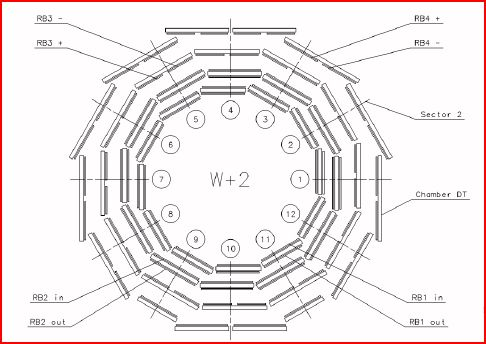
\includegraphics[width=0.8\textwidth]{barrel_layout}
    \hspace{1cm}
    \caption{Transverse view of the Barrel RPC system.}
    \label{fig:barrel_lay}
  \end{center}
\end{figure}

For each sector there are 4 DT stations, inserted in the 
iron gaps of the Barrel Yoke, from MB1 (the inner one)
to MB4 (the outer one). 

The RPC stations are mounted on one or both sides of the DT 
stations. Station MB1 is provided with RPC stations on 
bottom and top sides (RB1In and RB1Out stations), same 
for MB2 (RB2In and RB2Out stations). Stations MB3 and MB4
are provided with RPC stations on the bottom side only
(RB3 and RB4 stations). 
With this design, a total of six concentric RPC layers are 
available in the Barrel Muon System. The inner
layers can provide up to four coordinate measurements also for 
low momentum tracks crossing only MB1 and MB2 stations.

For each RPC station, pick-up strips running parallel to the 
beam axis provide coordinate measurement in the $r$-$\phi$ view,
thus allowing \pt measurement of the track. 
Segmentation in the $\eta$ view is obtained by sectioning
a plane of strips in two or three parts. 
The $\eta$ partitions are called {\em rolls}.
An RPC station can be segmented into two rolls (named Backward and 
Forward) or three rolls (named Backward, Middle, and Forward).
RPC stations 3 and 4 present also a segmentation along $\phi$ in two 
partitions ( named + and - ). RPC Station 4 sector 4 is segmented in 4 $\phi$ partitions.

\section{The L1 trigger system for Barrel RPCs}
From the point of view of the L1 trigger~\cite{ref:trig_tdr}, 
the RPC system volume is logically partitioned into 
sections. L1 trigger objects are searched 
for independently in each section.
Sections in the $\eta$ view will be referred as {\em towers},
and for each tower the partitions in  
in the $r$-$\phi$ view will be referred as {\em cones}.


\subsection{Trigger towers}
The definition of the $\eta$ boundaries 
of towers (see Fig.~\ref{fig:eta_towers}) is based on a set 
of reference layers.

\begin{figure}[hbtp]
  \begin{center}
    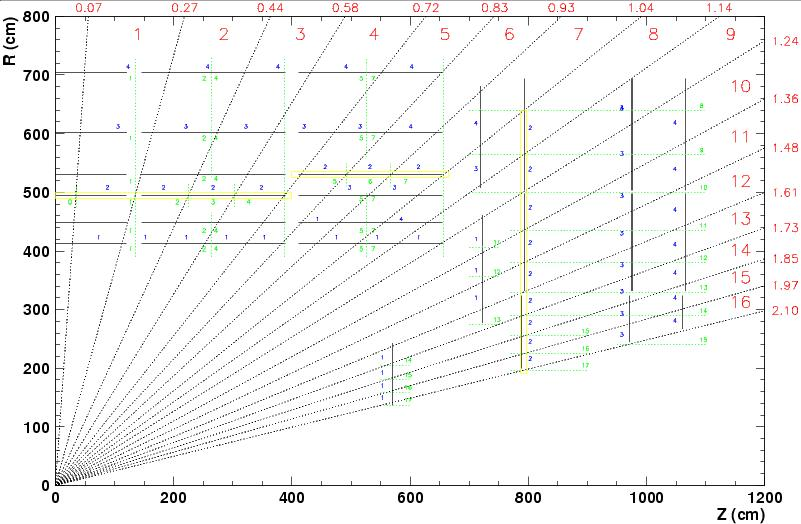
\includegraphics[width=0.8\textwidth]{eta_towers}
    \hspace{1cm}
    \caption{Trigger eta towers.}
    \label{fig:eta_towers}
  \end{center}
\end{figure}

In the Barrel, the reference layers are:
layer RB2In for W+1, W0, and W-1, 
and layer RB2Out for W-2 and W+2. 
Each tower must contain only one entire roll 
of a reference layer. On the 
other hand, a roll of a non-reference layer
can belong to adjacent towers, thus in this case 
the association of roll to towers is not univocally defined. 
The RPC trigger logic has a total of 17 towers.
A total of 5+5+1 towers are entirely contained in the Barrel.



\subsection{Trigger cones}
On the reference layers, the strips are grouped in
non-overlapping sets of 8 adjacent strips called {\em segments}.
Each segment subtends a $\phi$ angle of $2.5^\circ$, for a total 
of 144 segments (12 segments for each sector).
Each cone must contain only one segment of a reference 
layer.
On the other hand, in non-reference layers a larger number
of strips is grouped into a segment, so that a segment
covers more than $2.5^\circ$ in those layers.
Thus adjacent segments overlap in the non-reference layers and 
the association of a strip to those segments is not univocally defined.
% The cones appear more 
%like hourglass shaped partions.

\subsection{The L1 PACT logic}
The PAttern COmparator Trigger (PACT) logic 
collects RPC hits from all stations and searches for
spatial and time coincidences independently
in each cone. The $\eta$ and $\phi$ coordinate of the trigger
objects are assigned on the reference station.
By comparison with predefinite patterns of hits, 
also a \pt value is assigned to the candidate trigger 
object. Due to the overlap of adjacent cones, 
{\em ghost} trigger objects can appear. For this reason, 
the trigger objects found in a certain $\eta$ tower 
are processed by a proper ghost identification and removal logic,
and the remaining ones are sorted according to quality criteria.
 
Twelve logical sectors for the trigger system
are defined along the $r-\phi$ view. Those sectors are all
$30^\circ$ wide in $\phi$ and are shifted by 
$10^\circ$ with respect to the phisical sectors of the detector. % (see Fig. ~\ref{fig:trigger_sectors} ).

%\begin{figure}[hbtp]
%  \begin{center}
%    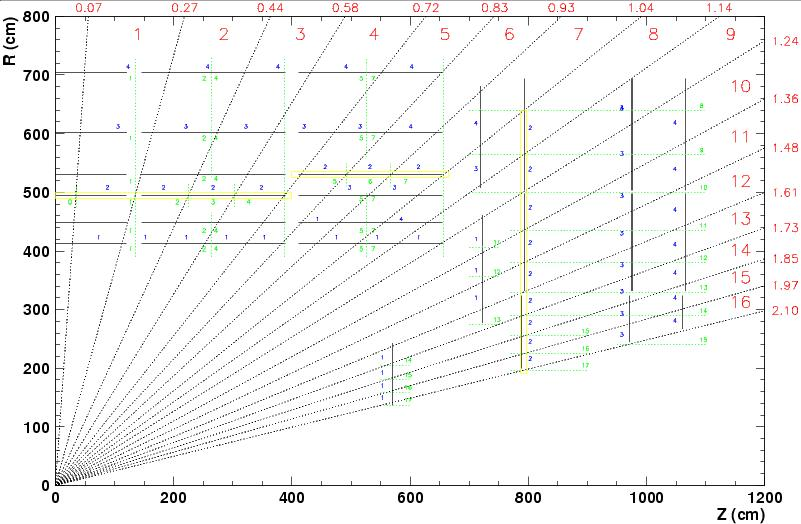
\includegraphics[width=0.8\textwidth]{eta_towers}
%    \hspace{1cm}
%    \caption{Trigger logical sectors vs detector physical sectors.}
%    \label{fig:trigger_sectors}
%  \end{center}
%\end{figure}



For each of those sectors a single muon candidate can be produced.
If more than one candidate is present, as in the case of a ghost the best one is selected 
according to quality criteria of the algorythm: number of hits,
type of layers fired and \pt of the track.  

Ghosts can also appear in adjacent towers and in adjacent logical sectors
due to the sharing of the rolls in non-reference stations. 


For this reason, trigger candidates from all the towers and sectors
 are further processed for ghosts removal, sorted according to 
quality criteria, and the 4 highest \pt muons
from the Barrel and the 4 highest \pt muons from the 
Endcap are finally sent to the Global Muon Trigger.

\subsection{Cosmic patterns in PACT}
In order to increase the trigger efficiency for 
cosmic muons, which are not constrained
to come from the interaction vertex, 
a looser pattern definition has been 
adopted with respect to collision runs.
A cosmic pattern is defined as a 
time coincidence of hits on at least
3 different RPC stations in a cone (3/6 majority).
No different patterns as a function 
of \pt are defined, thus the system is
not able to assign a \pt value 
to the track.

\section{Analysis method}
We start from a sample of reconstructed tracks 
in the Muon System which are matched to a DT 
trigger object. 
The track is required in order to reject fakes 
and to have an unambiguous association with a physics object.
The matching with the DT is done in order to select a sample 
that has not been triggered exclusively by RPCs.

If the number of tracks in the sample is 
$N_{match}^{DT}$, and under the assumption
that RPC and DT triggers are uncorrelated,
the RPC trigger efficiency 
$\epsilon_{L1}^{RPC}$ is given by the fraction 
of tracks in the sample that are matched also 
to an RPC trigger object:
\begin{equation}
\epsilon_{L1}^{RPC} = N_{match}^{RPC\&DT}/N_{match}^{DT} \,\,\,.
\end{equation}

\subsection{Tracks selection}
For the analysis we use a collection of CosmicMuons.
CosmicMuons are made of tracks reconstructed in the
Muon System only .
The two legs of a muon which traverses
the Tracker System are reconstructed as two separate 
CosmicMuon tracks.
%Kinematic parameters of a CosmicMuon track are given 
%at its {\em innermost position}. Not true anymore
%For tracks in the top part of the detector
%the innermost position is located on the outer stations
%(because the track is going from top to bottom),
%2Bwhile for tracks in the bottom part it is located 
%in the inner stations.
In order to prevent an eventual bias due to tracks 
that would not have been reconstructed without
RPC hits, we re-run the reconstruction using DT only.

We select cosmic tracks pointing to the $p$-$p$ interaction
region by requiring that the muons.
 
The above cuts are applied at skim level.
(definition of TrackerPointing skim).

In addition, we apply the following 
cuts:
\begin{itemize}
\item
$\pt$ at the innermost point $ > 5$GeV \ c 
\item
$N_{hits}$ in the DT $ > 20 $;
\item
$\chi^2$ of the track fit $ < 20 $.
\end{itemize}
The \pt cut removes tracks which are
looping in the transverse plane due 
to the magnetic field.%bending.
The last two cuts ensure good quality
of the DT reconstruction and 
prevent an eventual bias due to 
tracks that would not have been triggered 
without RPC hits.
Figures ~\ref{fig:pttrack}, ~\ref{fig:nhitschi2} show the distributions
of these variables for typical pointing
CosmicMuon tracks.

\subsection{Track matching with trigger objects}
The kinematic parameters of the track are the result of the reconstruction.
The position in $\eta - \phi$ of the L1 trigger for both DTs and RPCs is defined
on the reference layers. The DT reference layer is station 2 of each wheel.
In order to match the track to the trigger candidates the track
is extrapolated to the reference layer of the DTs.
The extrapolation is done by taking the last point of the track and propagating 
backwards to the reference Layer using {\em SteppingHelixPropagator},
an accurate propagation method through the CMS detector
geometry which takes into account the magnetic field, the 
energy loss in the detector material and the multiple scattering.

The distributions of $\eta$ and $\phi$ at the reference 
station for the tracks are shown in Fig. ~\ref{fig:track_eta_phi} 



\begin{figure}[hbtp]

 \begin{minipage}{1.0\textwidth}
  \begin{center}
 
     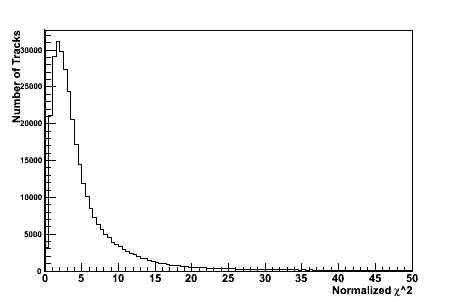
\includegraphics[width=0.4\textwidth]{chi2_sta}
     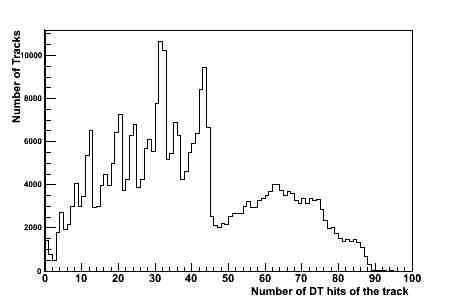
\includegraphics[width=0.4\textwidth]{num_hits_sta}
       % \caption{Distribution of the trigger efficiency vs $\eta$ and $\phi$ of the tracks on the reference layer for the top part of the detector ( y$ > $ 0 ).}
\caption{Distribution of the normalized $\chi^2$ (left) and number of DT hits (right) 
of the cosmic muon track. The tracks with < 5 hits
 are reconstructed through the CSCs chambers. }
      \label{fig:nhitschi2}
  \end{center}
  \end{minipage}

     \begin{minipage}{1.0\textwidth}
     \begin{center}
      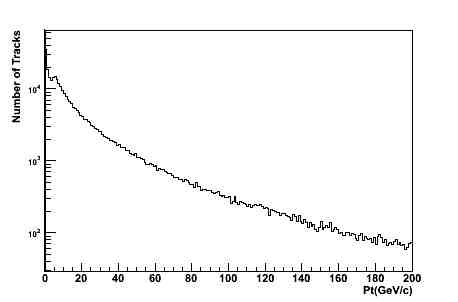
\includegraphics[width=0.8\textwidth]{pt_sta}
       \caption{ 
Distribution of the \pt of the cosmic muon tracks 
}
      \label{fig:pttrack}
%    \caption{Distribution of the trigger efficiency vs $\eta$ and $\phi$ of the tracks on the reference layer for the bottom part of the detector ( y $ < $ 0 ).}
  \end{center}
  \end{minipage}
     
%      \caption{Distribution of the \pt, normalized $\chi^2$ and number of hits in the DT chambers for the cosmic muon tracks }


\end{figure}


The track-trigger matching is performed in the $\phi$ coordinate 
only, which is the most accurate coordinate measured by both 
DT and RPC trigger systems. It was not possible to use a matching
in $\eta$ with the L1 DT trigger candidates since the $\eta$ part
of the algorythm was not commissioned yet during CRAFT08 data taking. 
The $\phi$ distributions for DT and
RPC triggers objects are shown in Fig. ~\ref{fig:trigger_eta_phi}

\begin{figure}[hbtp]
  \begin{center}
    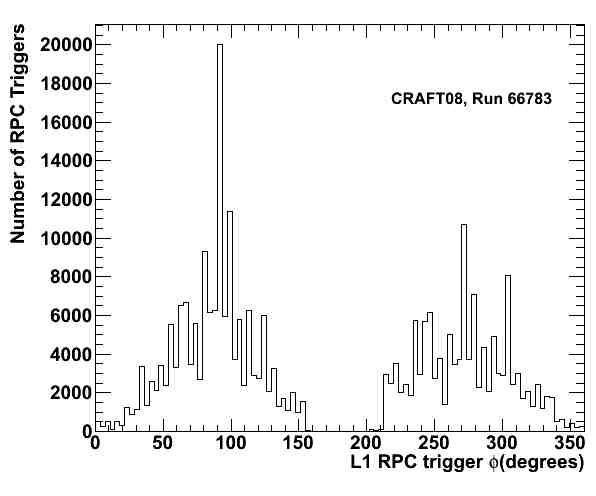
\includegraphics[width=0.4\textwidth]{phi_rpc}
    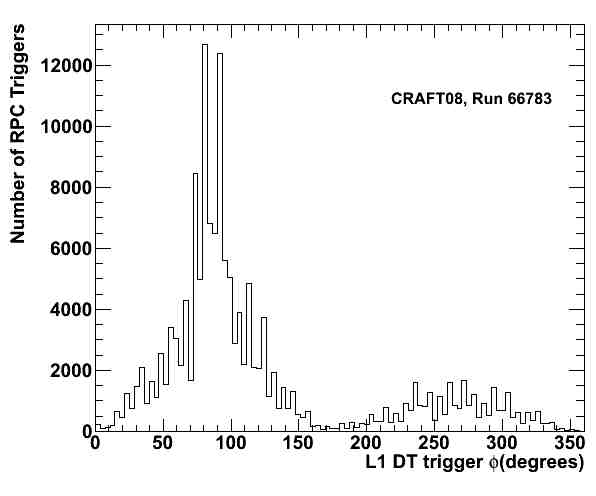
\includegraphics[width=0.4\textwidth]{phi_dt}
      \caption{Phi distribution of the RPC and DT triggers.}
    \label{fig:trigger_eta_phi}
  \end{center}
\end{figure}


We first match the track to a DT trigger.
The matching requirement is $|\Delta\phi_{t-DT}| < 30^\circ$,
where $\Delta\phi_{t-DT}$ is the difference 
between the $\phi$ of the track at the reference layer and
the $\phi$ of the DT trigger. This loose requirement
provides a high matching efficiency.


If we find a match with a DT trigger, then we proceed
for matching to an RPC trigger. 
Figure ~\ref{fig:trigger_residuals} shows the overall $\Delta\phi_{t-RPC}$ as measured 
using both cosmic patterns and collision patterns (the
last one obtained by running the trigger emulator).



\begin{figure}[hbtp]
  \begin{center}%
    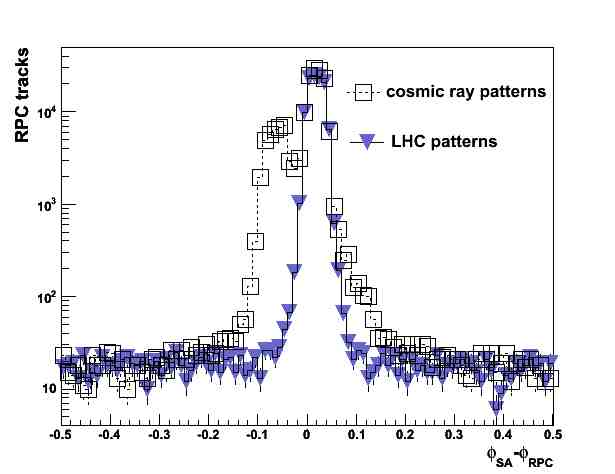
\includegraphics[width=0.8\textwidth]{residuals_rpc}
%    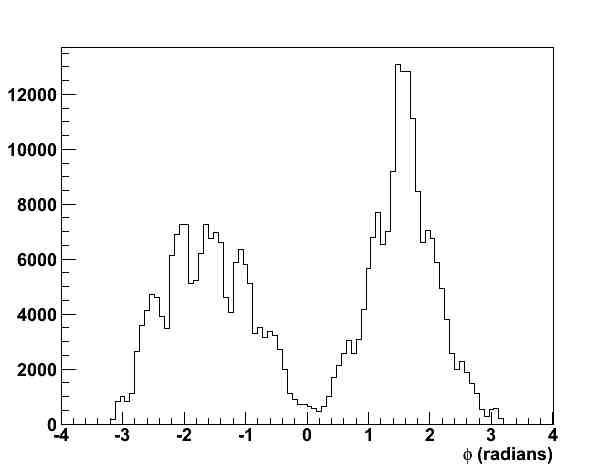
\includegraphics[width=0.8\textwidth]{phi_sta}
    \hspace{1cm}
    \caption{Distribution of the difference between the $\phi$ of the track measured at the reference station and the $\phi$ of the RPC trigger (Run 66783).}
    \label{fig:trigger_residuals}
  \end{center}
\end{figure}

The matching requirement is $|\Delta\phi_{t-RPC}| < 30^\circ$,
where $\Delta\phi_{t-RPC}$ is the difference 
between the $\phi$ of the track at the reference layer 
and the $\phi$ of the RPC trigger.

The second peak at $\phi  \tilde -6$ for the residuals distribution
 of cosmics patterns in Figure ~\ref{fig:trigger_residuals} is due
to the fact that the cosmics 
pattern configuration cannot identify the \pt of the track.
In case of  two candidates with the same quality then the one
with the smaller $\phi$ is selected.



\section{Data samples}
Only cosmic tracks which mimic muons from collisions
have been considered for this study. 
For this reason, we have analized runs taken from the 
following CRAFT08 and CRAFT09 datasets:
\begin{itemize}
\item
Commissioning08\/2213\_Tosca090322\_2pi\_scaled\_ReReco\_FromTrackerPointing-v1\/RAW-RECO
\item
Cosmics\/CRAFT09-PromptReco-v1\/RECO
\end{itemize}

The CRAFT08 dataset is a TrackerPointing skim, that is 
only cosmics pointing to the primary vertex 
region of CMS are selected. 
On the contrary, the CRAFT09 dataset is non-skimmed, 
since the pointing skim was not yet 
available. In this case we have filtered the 
events at the analysis level by applying the same
requirements used in the pointing skim.

Table~\ref{tab:runs} reports the run numbers analyzed and the detector
conditions.
 \begin{table}[htb]
    \label{tab:runs}
    \begin{center}
      \begin{tabular}{|c|c|c|c|} \hline
Dataset & Run   & RPC HV & FEB threshold \\ \hline
CRAFT08 & 66783 & 9.2 kV & 220 mV \\ \hline
CRAFT09 & 110409  & 9.4 kV & 220 mV \\ \hline
CRAFT09 & 110419  & 9.4 kV & 220 mV \\ \hline
      \end{tabular}
      \caption{Analyzed runs from CRAFT08 
and CRAFT09 datasets. The HV value and FEB thresholds for
the RPC system are also reported.}
    \end{center}
  \end{table}


\section{RPC trigger efficiency in CRAFT08}

For CRAFT08 a dataset was selected in which all the CMS Detector
 was included in the trigger. We studied the trigger efficiency 
with respect to the \pt of the track and with respect to the position 
of the track inside the detector.

Plots in Fig. ~\ref{fig:eff_eta_phi_08} show the efficiency of the trigger with respect to the 
position of the track extrapolated to the reference layer in the $\eta - \phi$
coordinates. The plot a shows the top part of the detector,
for $ 0^\circ < \phi < 180^\circ $ , 
the plot b shows the bottom part,

for  $ 180^\circ < \phi < 360^\circ $ , 


\begin{figure}[hbtp]

 \begin{minipage}{1.0\textwidth}
  \begin{center}
 
     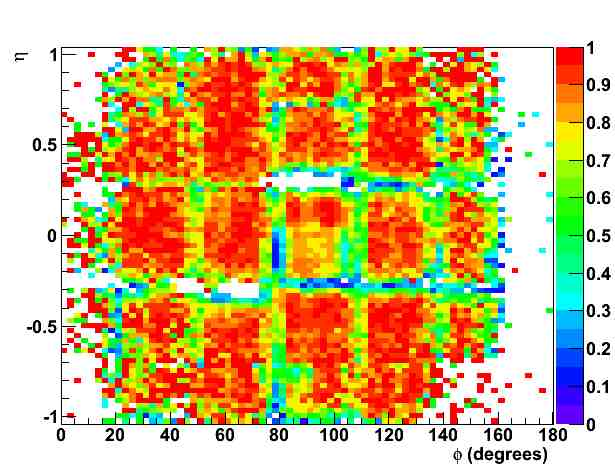
\includegraphics[width=0.8\textwidth]{eff_eta_phi_top_08}
       % \caption{Distribution of the trigger efficiency vs $\eta$ and $\phi$ of the tracks on the reference layer for the top part of the detector ( y$ > $ 0 ).}
       \caption{Top part of the detector (y$ > $ 0) }
  \end{center}
  \end{minipage}

     \begin{minipage}{1.0\textwidth}
     \begin{center}
      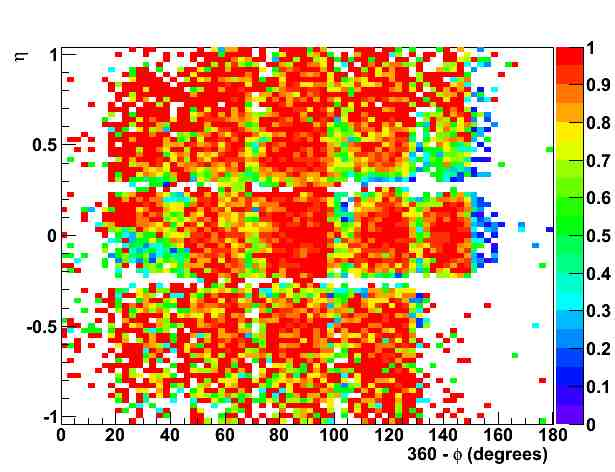
\includegraphics[width=0.8\textwidth]{eff_eta_phi_bot_08}
       \caption{Bottom part of the detector (y$ < $ 0) }
%    \caption{Distribution of the trigger efficiency vs $\eta$ and $\phi$ of the tracks on the reference layer for the bottom part of the detector ( y $ < $ 0 ).}
  \end{center}
  \end{minipage}
     
      \caption{Distribution of the trigger efficiency vs $\eta$ and $\phi$ of the tracks on the reference layer.}
      \label{fig:eff_eta_phi_08}

\end{figure}




From the plots it is possible to see the geometry of the RPCs on the reference layer 
in the Barrel.

For plot a, along the $\phi$ coordinate it is possible to see the sectors from 1 to 7.
The sector 1 and 7 are splitted in half through the two plots, since sector 1 covers the $\phi$
region from $-15\circ$ to $15\circ$. 

Along the $\eta$ coordinate it is possible to see separation between the five wheels. 

The inefficiency of the trigger is concentrated in the geometrical regions of the crack 
between the wheels and sectors.

%The plot Fig. ~\ref{fig:eff_eta_tower_08} shows the efficiency per $\eta$ tower. This integrates 
%over all the geometric inefficiencies in the $\phi$ direction.

%\begin{figure}[hbtp]
%  \begin{center}
%    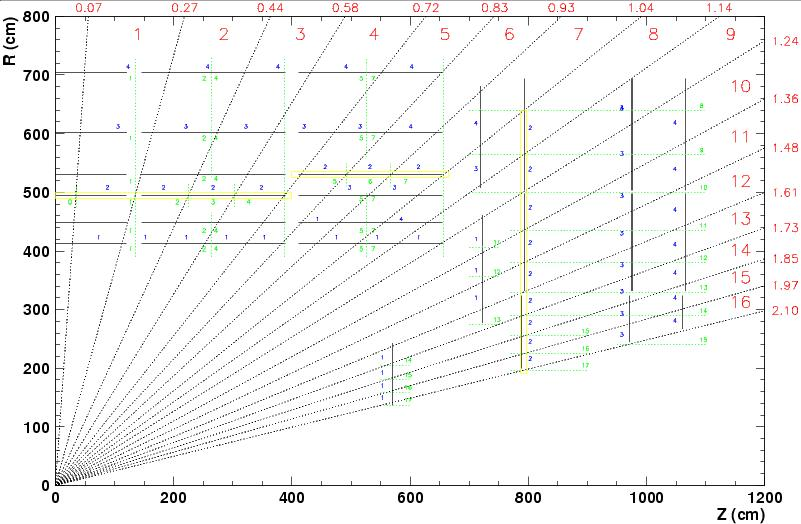
\includegraphics[width=0.8\textwidth]{eta_towers}
%2%B    \hspace{1cm}
%    \caption{Distribution of the trigger efficiency vs $\eta$ tower.}
%    \label{fig:eff_eta_tower_08}
%  \end{center}
%\end{figure}


The measurement of the efficiency for our method is based on the assumption that 
the DT trigger and the RPC trigger are independent.

In the region of the cracks between two sectors however the number of 
available patterns is limited and the DT and RPC trigger are correlated.

We introduced geometrical cuts in order to evaluate the trigger efficiency 
in the central regions of the rolls. 

The choice of the cuts is shown in table ~\ref{tab:volumecuts}. 




%Table~\ref{tab:volumecuts} reports the run numbers analyzed and the relevant
%conditions.

 \begin{table}[htb]
    \label{tab:volumecuts}
    \begin{center}
      \begin{tabular}{|c|c|} \hline
  $   |\phi - \phi_{center} | < 5^o $ & \\ \hline
  $  |z| < 100 or 200 < |z| < 300 or 450 < |z| < 550$  &  \\ \hline
      \end{tabular}
      \caption{Volume cuts applied to select the center of the sectors.
       $\phi_{center}$ is the value of $\phi$ at the center of the sector. 
}
    \end{center}
  \end{table}


The plot Fig. ~\ref{fig:eff_pt_08} shows the efficiency vs the $\pt$ of the cosmics tracks after 
the volu mecuts.

\begin{figure}[hbtp]
  \begin{center}
    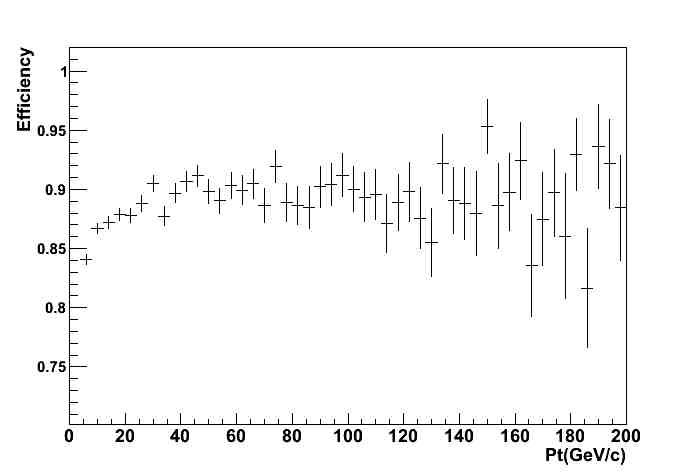
\includegraphics[width=0.8\textwidth]{eff_pt_08}
    \hspace{1cm}
    \caption{Distribution of the trigger efficiency vs \pt of the tracks.}
    \label{fig:eff_pt_08}
  \end{center}
\end{figure}


The efficiency gets in plateau after about \pt $\simeq 40 GeV/c$ . 


%The average efficiency in the fiducial volume is: 
%87.77 $\%$ $\pm 0.15$ 




A comparison has been made between this measurement and the measurement done in \cite{ref:mupaper}  %~\ref{antrigger}
with  the Tag \& Probe method.

The comparison was made on the top part of the detector,
 since the bottom part was used for the tagging:

 \begin{table}[htb]
    \label{tab:notecomparison}
    \begin{center}
      \begin{tabular}{|c|c|} \hline
Tag \& Probe: & $88.02 \pm 0.22 $ \\ \hline
DT vs RPC & $87.93 \pm 0.38 $  \\ \hline

%c < $\eta$ < d &  \\ \hline
     \end{tabular}
      \caption{Cuts applied for the comparison with the Tag $\and$ Probe method and values of the efficiency
}
    \end{center}
  \end{table}

%The cuts in the note TRIGGERREF were also applied for our analysis. in order to make 
%the comparison and the values obtained are reported in table ~\ref{tab:notecuts}

% \begin{table}[htb]
%5    \label{tab:notecuts}
%    \begin{center}
%2B      \begin{tabular}{|c|c|} \hline
%a < $\phi$ < b & \\ \hline
%c < $\eta$ < d &  \\ \hline
%      \end{tabular}
%2%B      \caption{Cuts applied for the comparison with the Tag $\and$ Probe method and values of the efficiency
%}
%    \end{center}
%  \end{table}



%The () choice of having separate plots for the top and bottom part of the detector
%is due to the 

\section{RPC trigger efficiency in CRAFT09}

For CRAFT09 a dataset was selected in which all the RPCs
 in the detector were included in the trigger. 

As for CRAFT08 the first study was made to 
measure the efficiency of the trigger as a function of $\eta - \phi$
of point of the track on the  reference layer( Fig ~\ref{fig:eff_eta_phi_09}). 


\begin{figure}[hbtp]

 \begin{minipage}{1.0\textwidth}
  \begin{center}
 
     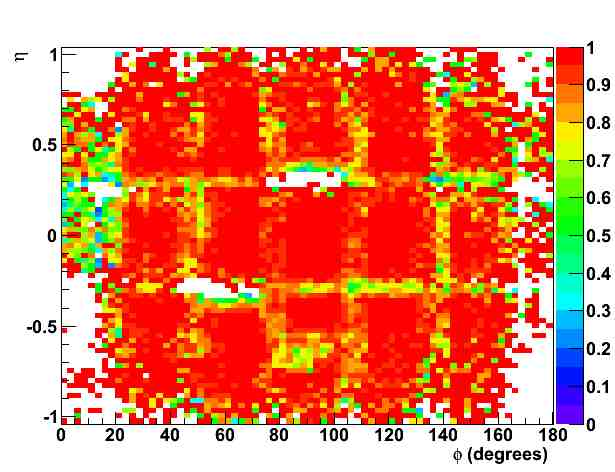
\includegraphics[width=0.8\textwidth]{eff_eta_phi_top_09}
       % \caption{Distribution of the trigger efficiency vs $\eta$ and $\phi$ of the tracks on the reference layer for the top part of the detector ( y$ > $ 0 ).}
       \caption{Top part of the detector (y$ > $ 0) }
  \end{center}
  \end{minipage}
     \begin{minipage}{1.0\textwidth}
     \begin{center}
      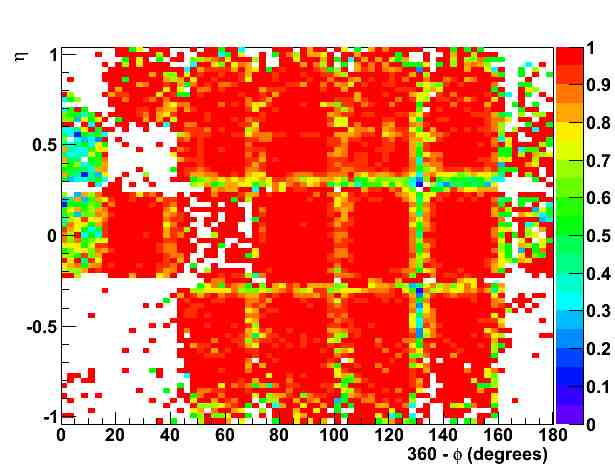
\includegraphics[width=0.8\textwidth]{eff_eta_phi_bot_09}
       \caption{Bottom part of the detector (y$ < $ 0) }
%    \caption{Distribution of the trigger efficiency vs $\eta$ and $\phi$ of the tracks on the reference layer for the bottom part of the detector ( y $ < $ 0 ).}
  \end{center}
  \end{minipage}
     
      \caption{Distribution of the trigger efficiency vs $\eta$ and $\phi$ of the tracks on the reference layer.}
      \label{fig:eff_eta_phi_09}

\end{figure}





%The plot Fig. ~\ref{fig:eff_eta_tower_09} shows the efficiency per $\eta$ tower.
%This integrates over all the geometric inefficiencies in the $\phi$ direction.

%\begin{figure}[hbtp]
 % \begin{center}
 %   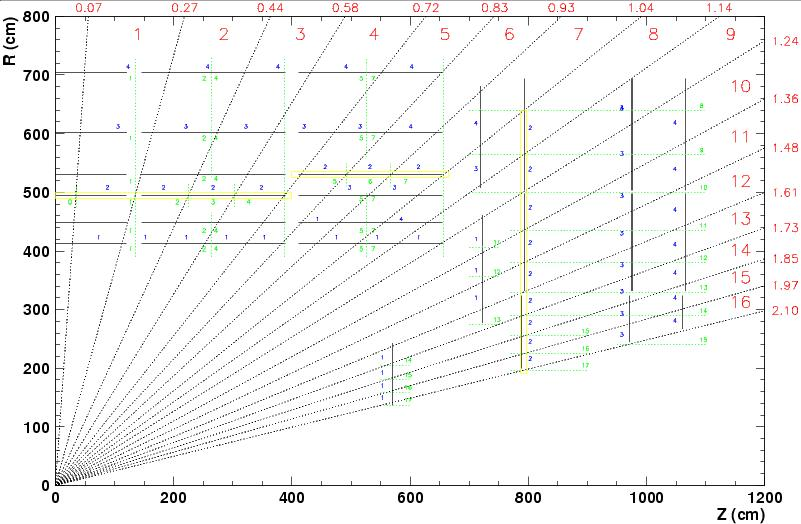
\includegraphics[width=0.8\textwidth]{eta_towers}
 %   \hspace{1cm}
 %   \caption{Distribution of the trigger efficiency vs $\eta$ tower.}
 %   \label{fig:eff_eta_tower_09}
 % \end{center}
%\end{figure}




The plot Fig. ~\ref{fig:eff_pt_09_vs_08} shows the efficiency vs the
\pt of the cosmics tracks after the cuts shown in table
~\ref{tab:volumecuts}. On the same plot it is shown 
the efficiency of CRAFT08 for a comparison.
An explaination for the difference between the efficiencies
is given in section FIXME 


\begin{figure}[hbtp]
  \begin{center}
    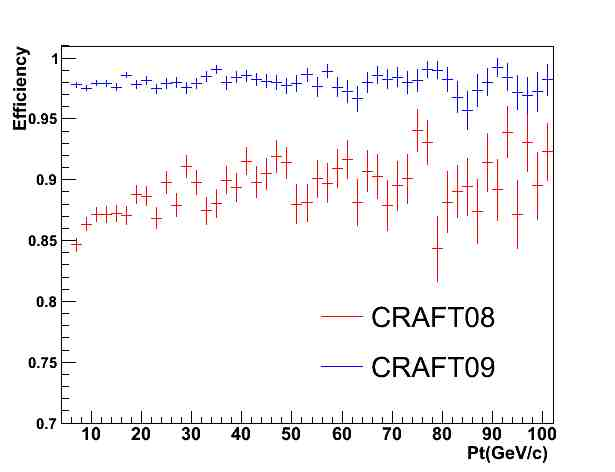
\includegraphics[width=0.8\textwidth]{eff_pt_09_vs_08}
    \hspace{1cm}
    \caption{Distribution of the trigger efficiency vs \pt of the tracks.}
    \label{fig:eff_pt_09_vs_08}
  \end{center}
\end{figure}


The efficiency for CRAFT09 is already in plateau at after the cut.% \pt $\simeq 20 GeV/c$ . 


%The average efficiency in the fiducial volume is:
% 95,9 $\%$ $\pm$ 




\section{Discussion: CRAFT08 vs. CRAFT09}


The plot in Fig ~\ref{fig:eff_pt_09_vs_08} shows the comparison between 
the trigger efficiency vs \pt in CRAFT08 vs CRAFT09.
%The comparison is done after the choice of volume cuts in Table ~\ref{tab:volumecuts} .

%\begin{figure}[hbtp]
%  \begin{center}
%    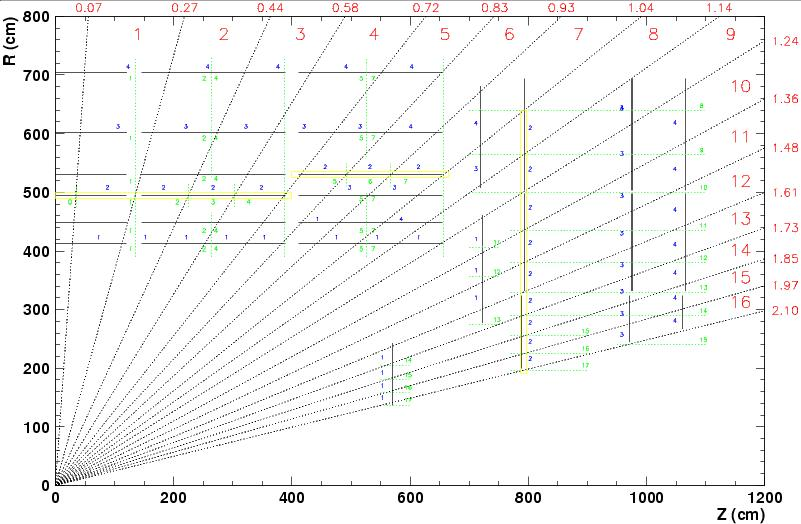
\includegraphics[width=0.8\textwidth]{eta_towers}
%    \hspace{1cm}
%    \caption{Distribution of the trigger efficiency vs \pt of the tracks.}
%    \label{fig:eff_pt_09_vs_08}
%  \end{center}
%\end{figure}


This plot shows a differnce of about $7-8 \% $  in the efficiency plateau region.

%In the case where all the RPCs have the same efficiency, 

Some considerations can be done to explain this difference.

In the cosmics pattern configuration the trigger is basically
a majority of 3 over 6 ( or 3 over 5) layers fired in the
same logical cone( see section FIXME ).

For a given a track in the muon system,
the number of hits in a logical cone
depends from the geometry of the cone and 
from the intrinsic efficiency of the RPC chambers

\subsection{The difference in detector efficiency }

Table ~\ref{tab:meaneffs} reports the mean values the efficiency 
for the barrel chambers for the two runs considered.

The increase in the RPC efficiency is due to the increase of the 
voltage from $9.2$ to $9.4$ kV and to the fixing of many problems 
of the detector done during CRAFT08 (see also \cite{ref:craft08pap} ).

The fourth column is the probability of having 3 layers fired
in the $``best''$ case where a track has 
geometrically crossed 6 out of 6 layers inside a 
logical cone ( $\epsilon_{6}$)
The fifth column is the 
probability of having 3 layers fired
in the  $ ``worst''$ case where
a track has geometrically crossed 3 out of 6 layers inside a 
logical cone ( $\epsilon_{3}$ ).
This calculation has been done
assuming that all detectors had efficiency equals to mean efficiency.


\begin{table}[htb]
  \label{tab:meaneffs}
    \begin{center}
      \begin{tabular}{|c|c|c|c|c|} \hline
Run & Mean efficiency in the Barrel & Voltage & $\epsilon_{6}$ & $\epsilon_{3}$\\ \hline
11409 &	$92.96 \%$ & 9.4 & $99.97 \%$ & $77.86 \%$  \\ \hline
66783 & $83.11 \%$ & 9.2 & $99.2 \%$ & $57.17 \%$ \\ \hline
      \end{tabular}
         \caption{ Mean efficiency of the chambers in the barrel, voltage and trigger efficiency in the $``best''$ case and in the $``worst''$ case 
}
 \end{center}
\end{table} 

We can see that in the $ ``best'' $ case the 
difference of the detector efficiency changes the $\epsilon_{trigger}$ 
by less than $1\%$.
In the  $ ``worst''$ case the $\epsilon_{trigger}$ changes by more than $20\%$.


The trigger efficiency will also take into account
all the intermediate cases, depending on the geometry of the cones. 

\subsection{The dependence on the cone geometry}

In order to quantitatively evaluate the weight of all possible cases,
the trigger efficiency in a given logical cone should be evaluated as:

\begin{equation}
\label{efficiency}
\epsilon_{trigger} = \sum_{i=3}^{i=6(5)}\prod_{combination j of i detectors} \epsilon_{geom,i,j} * \epsilon_{RPC,i,j}    
\end{equation} 
\\

where:\\
\begin{itemize}
\item $\epsilon_{geom,i,j}$ is the geometric acceptance of
 the cone for the combination $j$ of $i$ detectors
\item $\epsilon_{RPC,i,j}$ is the the probability that 
at least 3 RPC layers were fired amongst the $i$ detectors
geometrically intersected by the track
\end{itemize}


In order to quantitatively measure the weight of geometric factors
$\epsilon_{geom,i,j}$ further studies need to be done. 

%So the critical dependence we observe
%of the trigger efficiency from
%the efficiency of the chambers 

%This means that even if a track is reconstructed and it 
%has fired more than 3 RPC layers, it will not generate
%a L1 Trigger candidate if there are not 3 hits in the same
%logical cone.

However, we can observe that the logical cones
are optimized for tracks strictly pointing to
the interaction point. The pointing skim 
for  cosmics only requires that the tracks
are passing through the geometrical region of the tracker ( see section FIXME ).

This is a feature that is deeply embedded in the trigger electronics,
so it would have been impossible to change it for cosmics data taking.



\Section{Conclusions}

A method to measure the L1 RPC trigger efficiency has been developed.
It has been applied on cosmics data from CRAFT08 and 09, showing a significative 
improvement of the trigger efficiency.

The algorythm has already been included in the RPC Prompt Analysis framework.




The method has been indirectly validated
 through a comparison with the Tag and Probe 
method on CRAFT08 data, showing reasonable 
agreement between the two methods in the fiducial 
region described in section FIXME.


The main features of this algorythm are the following:

\begin{itemize} 
\item It can be used to measure the efficiency for channels
 where there are not 2 muons back to back ( all W channels, Top channel etc )
\item It can be adapted to measure the DT and CSC trigger efficiency.
\item It might present a bias in the non-fiducial regions. This matter has still 
to be investigated.
\end{itemize} 


Further validation can be done on MonteCarlo by comparing its 
results with MC truth.

%% References
\bibliography{auto_generated}

%
%\begin{figure}[hbtp]
%  \begin{center}
%    \includegraphics[width=0.2\textwidth]{CMS-bw-logo}\hspace{1cm}
\includegraphics[width=0.2\textwidth]{CMScol}
%    \hspace{1cm}
%    \caption{Figures inserted using includegraphics.}
%    \label{fig:ex1}
%  \end{center}
%\end{figure}

